\documentclass[aspectratio=43]{beamer}
\usepackage{slides}


\title{CU Denver Math Camp - Matrix Algebra}
\date{\today}
\author{Kyle Butts}

\definecolor{alice}{RGB}{0,114,178}
\definecolor{ruby}{HTML}{EB0E09}
\definecolor{yellow}{RGB}{240,228,66}
\definecolor{kelly}{RGB}{0,158,115}
\definecolor{maroon}{HTML}{AF3335}
\definecolor{cranberry}{HTML}{7E90B8}

\begin{document}
\maketitle

% Fundamentals 
\section{Matrix Fundamentals}

\begin{frame}{Matrix Fundamentals}
  \begin{center}
    $A = \begin{bmatrix}
        a_{11} & a_{12} & a_{13} \\
        a_{21} & a_{22} & a_{23} \\
      \end{bmatrix}$
  \end{center}

  \begin{itemize}
    \item A \alert{matrix} is a rectangular array of numbers.

    \item \alert{Size}/\alert{Dimension}: (rows) $\times$ (columns). E.g. $A$ is a $2 \times 3$ matrix.

          \begin{itemize}
            \item I remember by "Row your boat".
          \end{itemize}

    \item The element in row $i$ and column $j$ is referruby to as $a_{ij}$ or $A_{ij}$.
  \end{itemize}
\end{frame}

\begin{frame}{Matrix Addition and Subtraction}
  \begin{center}
    $A = \begin{bmatrix}
        {\color{ruby} a_{11}} & {\color{ruby} a_{12}} & {\color{ruby} a_{13}} \\
        {\color{ruby} a_{21}} & {\color{ruby} a_{22}} & {\color{ruby} a_{23}} \\
      \end{bmatrix}$ and $B = \begin{bmatrix}
        {\color{alice} b_{11}} & {\color{alice} b_{12}} & {\color{alice} b_{13}} \\
        {\color{alice} b_{21}} & {\color{alice} b_{22}} & {\color{alice} b_{23}} \\
      \end{bmatrix}$
  \end{center}

  \begin{itemize}
    \item Dimensions must match: $$
            ({\color{kelly} r} \times {\color{cranberry} c}) \pm ({\color{kelly} r} \times {\color{cranberry} c}) \implies ({\color{kelly} r} \times {\color{cranberry} c})
          $$

    \item $A$ and $B$ are both $2 \times 3$ matrices, so we can add and subtract them: \begin{center}
            $A \pm B = \begin{bmatrix}
                {\color{ruby} a_{11}} \pm {\color{alice} b_{11}} & {\color{ruby} a_{12}} \pm {\color{alice} b_{12}} & {\color{ruby} a_{13}} \pm {\color{alice} b_{13}} \\
                {\color{ruby} a_{21}} \pm {\color{alice} b_{21}} & {\color{ruby} a_{22}} \pm {\color{alice} b_{22}} & {\color{ruby} a_{23}} \pm {\color{alice} b_{23}} \\
              \end{bmatrix}$
          \end{center}


  \end{itemize}
\end{frame}

\begin{frame}{Scalar Multiplication}
  \begin{center}
    $A = \begin{bmatrix}
        a_{11} & a_{12} & a_{13} \\
        a_{21} & a_{22} & a_{23} \\
      \end{bmatrix}$
  \end{center}

  \begin{itemize}
    \item For any scalar $c$ (a number like 2 or -4): $$
            {\color{ruby} c} A = \begin{bmatrix}
              {\color{ruby} c} * a_{11} & {\color{ruby} c} * a_{12} & {\color{ruby} c} * a_{13} \\
              {\color{ruby} c} * a_{21} & {\color{ruby} c} * a_{22} & {\color{ruby} c} * a_{23} \\
            \end{bmatrix}$$

  \end{itemize}
  \begin{center}

  \end{center}

\end{frame}

\begin{frame}{Matrix Multiplication}
  \begin{center}
    $A = \begin{bmatrix}
        {\color{ruby} a_{11}}      & {\color{ruby} a_{12}}      & {\color{ruby} a_{13}}      \\
        {\color{cranberry} a_{21}} & {\color{cranberry} a_{22}} & {\color{cranberry} a_{23}} \\
      \end{bmatrix}$ and $D = \begin{bmatrix}
        {\color{alice} d_{11}} & {\color{kelly} d_{12}} \\
        {\color{alice} d_{21}} & {\color{kelly} d_{22}} \\
        {\color{alice} d_{31}} & {\color{kelly} d_{32}} \\
      \end{bmatrix}$
  \end{center}

  \begin{itemize}
    \item Inner Dimensions must match: $$
            ({\color{ruby} r} \times \underline{\color{alice} c}) \times (\underline{\color{alice} c} \times {\color{kelly} p}) \implies ({\color{ruby} r} \times {\color{kelly} p})
          $$

    \item $A$ is a $2 \times 3$ and $D$ is a $3 \times 2$ matrix, so we can multiply (the 2s are equal): \begin{center}
            $A \times D = \begin{bmatrix}
                {\color{ruby} a_{11}} {\color{alice} d_{11}} + {\color{ruby} a_{12}} {\color{alice} d_{21}} + {\color{ruby} a_{13}} {\color{alice} d_{31}}                & {\color{ruby} a_{11}} {\color{kelly} d_{12}} + {\color{ruby} a_{12}} {\color{kelly} d_{22}} + {\color{ruby} a_{13}} {\color{kelly} d_{32}}                \\

                {\color{cranberry} a_{11}} {\color{alice} d_{11}} + {\color{cranberry} a_{12}} {\color{alice} d_{21}} + {\color{cranberry} a_{13}} {\color{alice} d_{31}} & {\color{cranberry} a_{11}} {\color{kelly} d_{12}} + {\color{cranberry} a_{12}} {\color{kelly} d_{22}} + {\color{cranberry} a_{13}} {\color{kelly} d_{32}} \\
              \end{bmatrix}$
          \end{center}
  \end{itemize}

\end{frame}

\begin{frame}{Matrix Multiplication}
  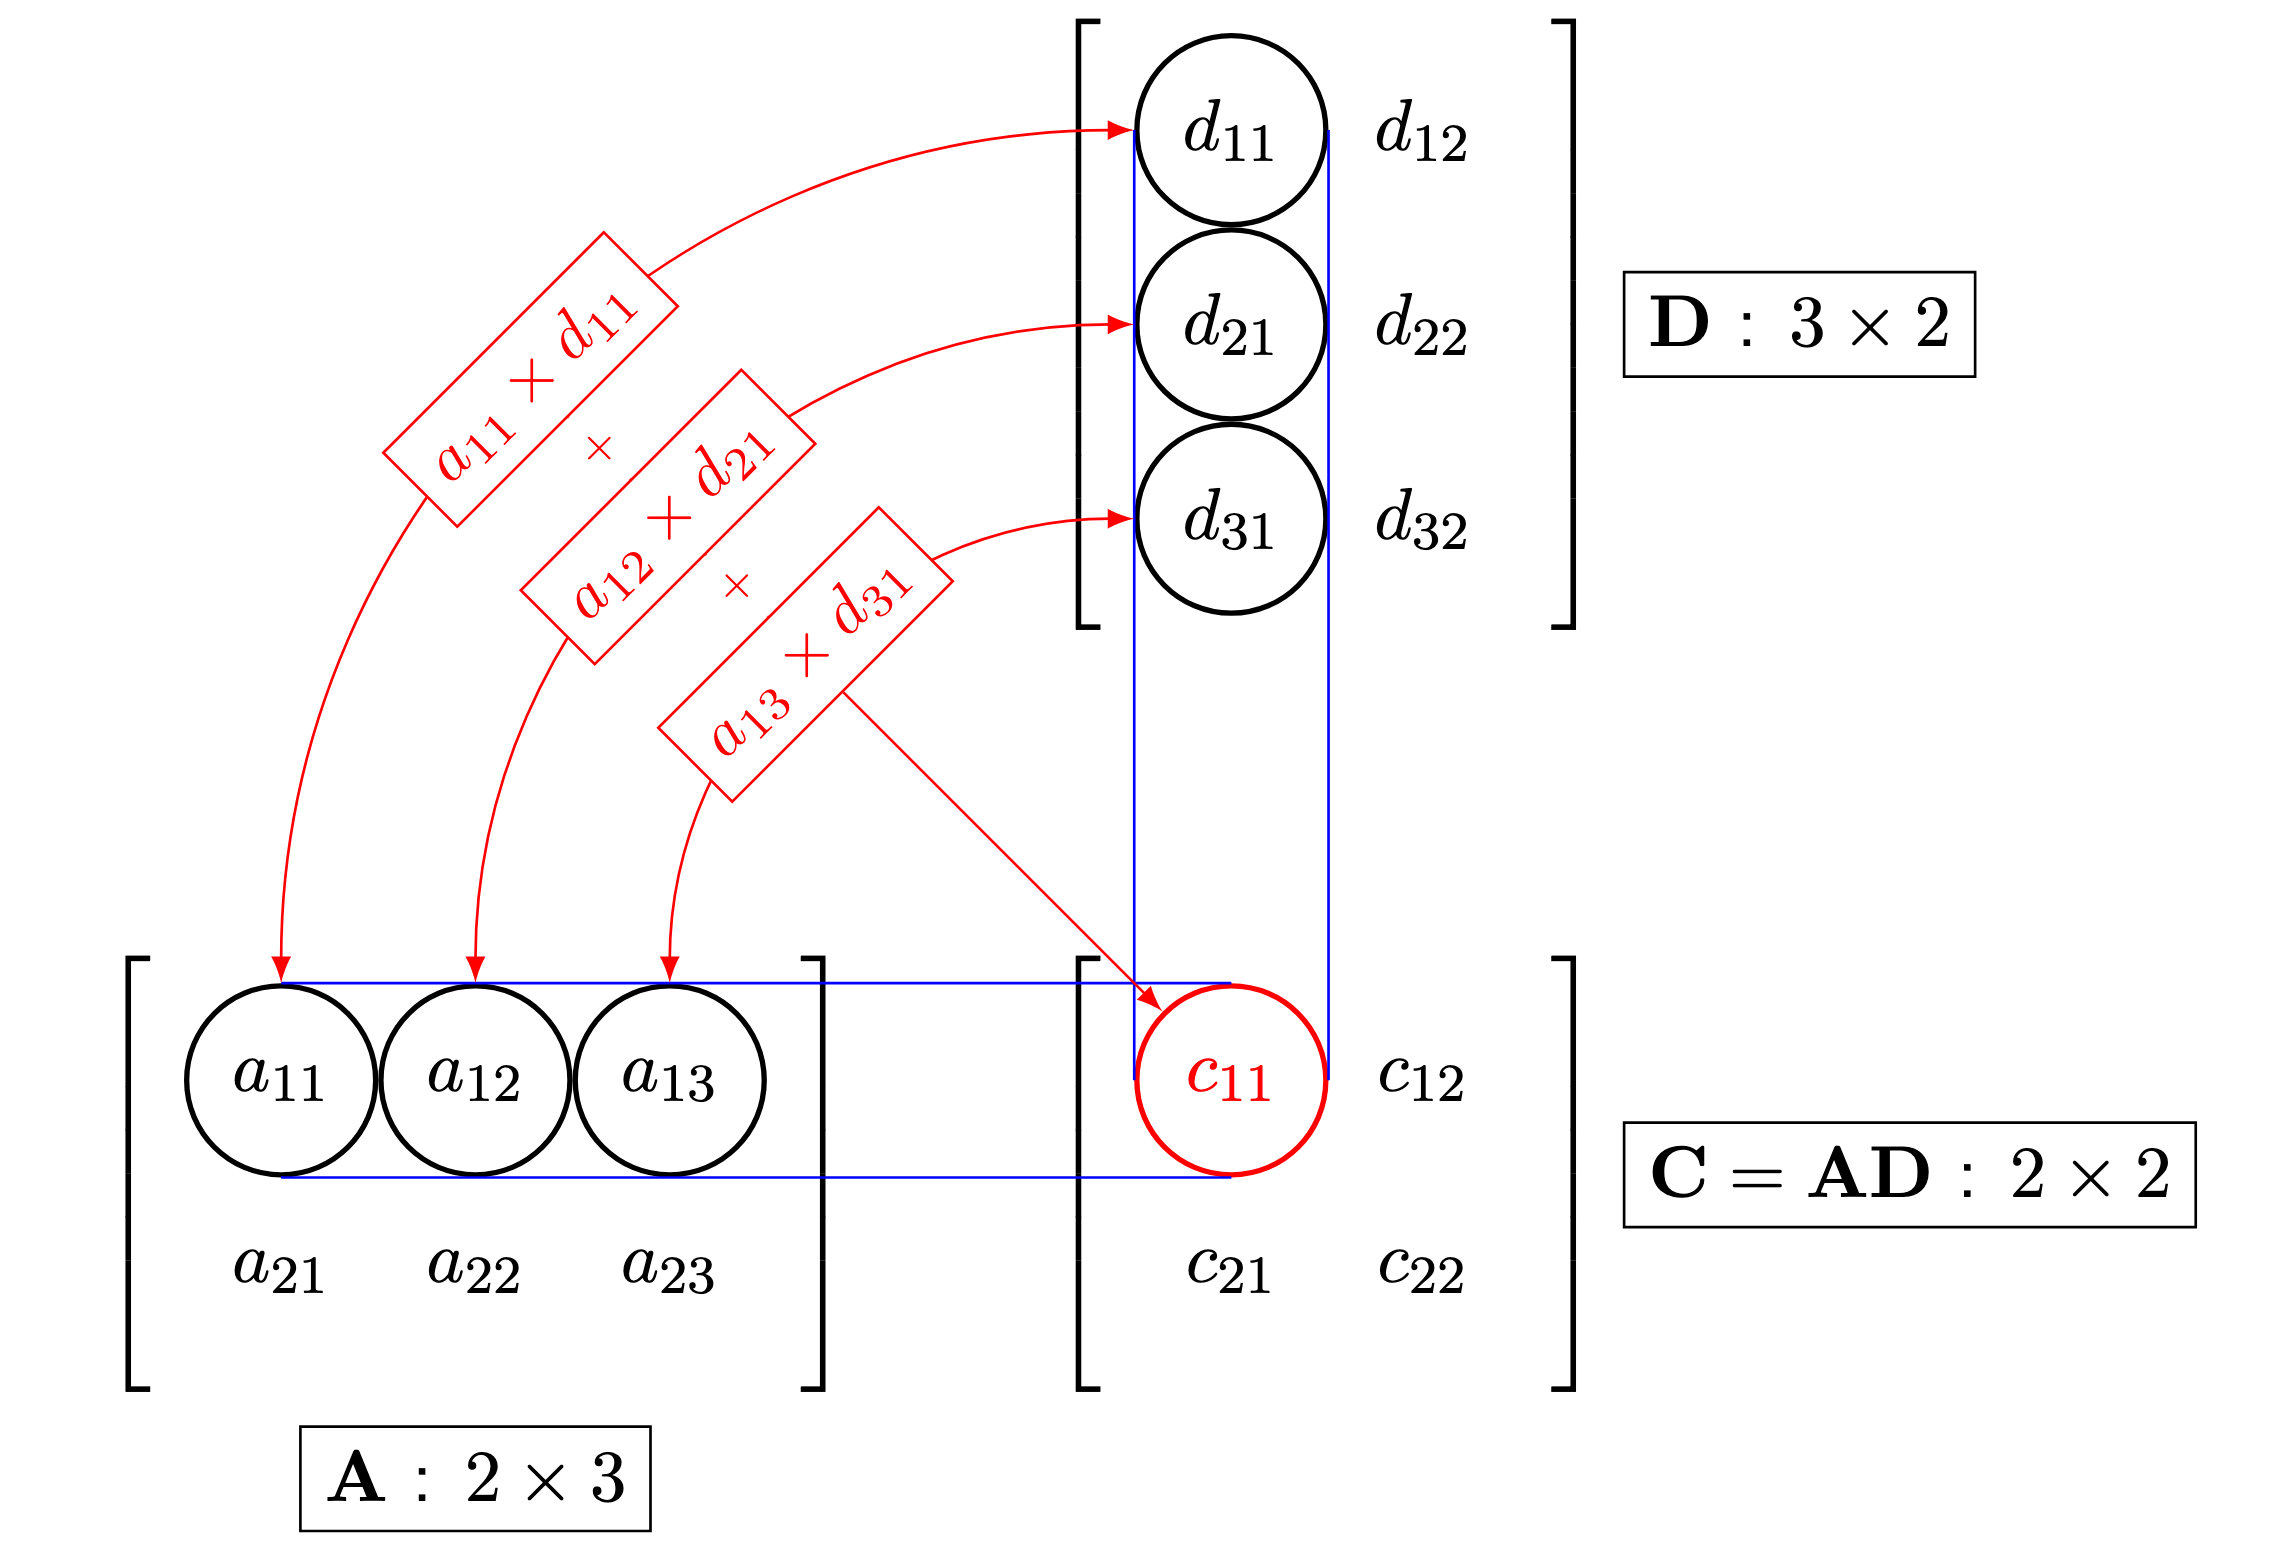
\includegraphics[width= \linewidth]{Matrix Multiplication.png}
\end{frame}



\begin{frame}{Matrix Multiplication Practice}
  \begin{center}
    $A = \begin{bmatrix}
        1 & 4 & 1 \\
        2 & 3 & 2 \\
      \end{bmatrix}$ and $B = \begin{bmatrix}
        1 & 1 \\
        2 & 1 \\
        2 & 2 \\
      \end{bmatrix}$
  \end{center}

  \begin{itemize}
    \item What is $A \times B$? What is $B \times A$?
  \end{itemize}

  \vspace{40mm}
\end{frame}

\begin{frame}{Transpose}
  $$
    A = \begin{bmatrix}
      {\color{ruby} x_1} & {\color{cranberry} y_1} & {\color{alice} z_1} \\
      {\color{ruby} x_2} & {\color{cranberry} y_2} & {\color{alice} z_2} \\
    \end{bmatrix}
  $$

  \begin{itemize}
    \item The \alert{tranpose} of an $n \times m$ matrix $A$, labelled $A^T$ or $A'$, is a $m \times n$ matrix, where the columns in $A$ are the rows in $A^T$.
  \end{itemize}

  $$
    A^T = \begin{bmatrix}
      {\color{ruby} x_1}      & {\color{ruby} x_2}      \\
      {\color{cranberry} y_1} & {\color{cranberry} y_2} \\
      {\color{alice} z_1}     & {\color{alice} z_2}     \\
    \end{bmatrix}
  $$
\end{frame}

\begin{frame}{Transpose Practice}
  \begin{center}
    $A = \begin{bmatrix}
        1 & 4 & 1 \\
        2 & 3 & 2 \\
      \end{bmatrix}$ and $B = \begin{bmatrix}
        1 & 1 \\
        2 & 1 \\
        2 & 2 \\
      \end{bmatrix}$
  \end{center}

  \begin{itemize}
    \item What is the transpose of $A$ and $B$?
  \end{itemize}
\end{frame}

\begin{frame}{Variance Covariance Matrix}
  \begin{itemize}
    \item Consider a matrix of variable where each column is a (de-meaned) sample.
          $$
            A = \begin{bmatrix}
              {\color{ruby} x_1 - \bar{x}} & {\color{cranberry} y_1 - \bar{y}} & {\color{alice} z_1 - \bar{z}} \\
              {\color{ruby} x_2 - \bar{x}} & {\color{cranberry} y_2 - \bar{y}} & {\color{alice} z_2 - \bar{z}} \\
              \vdots                       & \vdots                            & \vdots                        \\
              {\color{ruby} x_n - \bar{x}} & {\color{cranberry} y_n - \bar{y}} & {\color{alice} z_n - \bar{z}} \\
            \end{bmatrix},
          $$ where $\bar{x}$ is the mean of variable $x$.
  \end{itemize}
\end{frame}

\begin{frame}{Variance Covaraince Matrix}
  \begin{itemize}
    \item The Variance-Covariance Matrix is $A^T A = $

          $${\footnotesize
                \begin{bmatrix}
                  \sum_{i=1}^n {\color{ruby} (x_i - \bar{x})}^2                                  & \sum_{i=1}^n {\color{ruby} (x_i - \bar{x})}{\color{cranberry} (y_i - \bar{y})}  & \sum_{i=1}^n {\color{ruby} (x_i - \bar{x})}{\color{alice} (z_i - \bar{z})}      \\
                  \sum_{i=1}^n {\color{cranberry} (y_i - \bar{y})}{\color{ruby} (x_i - \bar{x})} & \sum_{i=1}^n {\color{cranberry} (y_i - \bar{y})}^2                              & \sum_{i=1}^n {\color{cranberry} (y_i - \bar{y})}{\color{alice} (z_i - \bar{z})} \\
                  \sum_{i=1}^n {\color{alice} (z_i - \bar{z})}{\color{ruby} (x_i - \bar{x})}     & \sum_{i=1}^n {\color{alice} (z_i - \bar{z})}{\color{cranberry} (y_i - \bar{y})} & \sum_{i=1}^n {\color{alice} (z_i - \bar{z})}^2                                  \\
                \end{bmatrix}
              }
          $$
          $$
            = \begin{bmatrix}
              Var({\color{ruby} x})                       & Cov({\color{ruby} x},{\color{cranberry} y})  & Cov({\color{ruby} x},{\color{alice} z})      \\
              Cov({\color{cranberry} y},{\color{ruby} x}) & Var({\color{cranberry} y})                   & Cov({\color{cranberry} y},{\color{alice} z}) \\
              Cov({\color{alice} z},{\color{ruby} x})     & Cov({\color{alice} z},{\color{cranberry} y}) & Var({\color{alice} z})                       \\
            \end{bmatrix}
          $$
  \end{itemize}
\end{frame}

% Transformations and their Inverses
\section{Transformations and their Inverses}

\begin{frame}{Vectors}
  \begin{itemize}
    \item Vectors are matrices with only one row or column. For example,the column vector: $$
            \vec{x} = \begin{bmatrix} x_1 \\ x_2 \\ \vdots \\ x_n \end{bmatrix}
          $$


    \item You can think of vectors as being a line in $\mathbb{R}^n$.

    \item For example, any point on $x$-$y$ plane can be written as a $2 \times 1$ vector:$$
            \begin{bmatrix} 0 \\ 1 \end{bmatrix} \text{ and } \begin{bmatrix} 2 \\ 3 \end{bmatrix}
          $$
  \end{itemize}

\end{frame}

\begin{frame}{Matrix Times a Vector (Transformations)}
  $$A = \begin{bmatrix}
      {\color{ruby} a_{11}}  & {\color{kelly} a_{12}}     \\
      {\color{alice} a_{21}} & {\color{cranberry} a_{22}}
    \end{bmatrix} \text{ and } x = \begin{bmatrix} x_1 \\ x_2 \end{bmatrix}$$

  \begin{itemize}
    \item An $n \times n$ matrix, $A$, times a $n \times 1$ vector, $x$, is a transformation from $\mathbb{R}^n$ to $\mathbb{R}^n$. So $A$ takes $x$, rotates it around and/or shrinks or extends the line.

    \item In general, $$
            Ax = \begin{bmatrix}
              {\color{ruby} a_{11}} x_1 + {\color{kelly} a_{12}} x_2      \\
              {\color{alice} a_{21}} x_1 + {\color{cranberry} a_{22}} x_2
            \end{bmatrix} \in \mathbb{R}^2
          $$
  \end{itemize}
\end{frame}




\begin{frame}{Identity Matrix (A Special Transformation)}
  \begin{center}
    $I_n = \begin{bmatrix}
        1      & 0      & 0      & \dots  & 0      \\
        0      & 1      & 0      & \dots  & 0      \\
        0      & 0      & 1      & \dots  & 0      \\
        \vdots & \vdots & \vdots & \ddots & \vdots \\
        0      & 0      & 0      & \dots  & 1
      \end{bmatrix} $
  \end{center}

  \begin{itemize}
    \item This matrix has a special property. It is the matrix equivalent to $1$.

    \item If you multiply a matrix of "conformable" size with the identity matrix, it returns the original matrix.

    \item Example: $$
            \begin{bmatrix} 1 & 0 \\ 0 & 1 \end{bmatrix} \times
            \begin{bmatrix} 2 \\ 3 \end{bmatrix} =
            \begin{bmatrix} 1*2 + 0*3 \\ 0*2 + 1*3 \end{bmatrix} =
            \begin{bmatrix} 2 \\ 3 \end{bmatrix}
          $$
  \end{itemize}
\end{frame}

\begin{frame}{Transformation Examples}
  \begin{itemize}
    \item Reflection on the Y-axis: $$
            \begin{bmatrix} -1 & 0 \\ 0 & 1\end{bmatrix} \begin{bmatrix} x \\ y \end{bmatrix} = \begin{bmatrix} -x \\ y \end{bmatrix}
          $$

    \item Reflection  90 degrees clockwise: $$
            \begin{bmatrix} 0 & 1 \\ -1 & 0\end{bmatrix} \begin{bmatrix} x \\ y \end{bmatrix} = \begin{bmatrix} y \\ -x \end{bmatrix}
          $$

    \item Enlargement by scale factor $a$ in the $x$ direction and scale factor $b$ in the $y$ direction: $$
            \begin{bmatrix} a & 0 \\ 0 & b \end{bmatrix} \begin{bmatrix} x \\ y \end{bmatrix} = \begin{bmatrix} ax \\ by \end{bmatrix}
          $$
  \end{itemize}
\end{frame}

\begin{frame}{Combination of Transformations}
  \begin{itemize}
    \item Let's say I want to rotate a vector 90 degrees clockwise and then keep only the $x$ direction (i.e. scale the $y$ by $0$.)

    \item I just multiply the matrices in the order I want to do them:

          $$
            \underbrace{\begin{bmatrix} 1 & 0 \\ 0 & 0 \end{bmatrix}}_{\text{Keep only } x} \overbrace{\begin{bmatrix} 0 & 1 \\ -1 & 0 \end{bmatrix}}^{\text{Rotate 90 degrees clockwise}} \begin{bmatrix} x \\ y \end{bmatrix} = \begin{bmatrix} 1 & 0 \\ 0 & 0 \end{bmatrix} \begin{bmatrix} y \\ -x \end{bmatrix} = \begin{bmatrix} y \\ 0 \end{bmatrix}
          $$
  \end{itemize}
\end{frame}

\begin{frame}{Determinant of a Matrix}
  \begin{itemize}
    \item When we rotate and scale an image, we are just doing many many vectors times a transformation matrix. The determinant asks how much does the area change with out transformation:

          \vspace{5mm}
          \begin{center}
            
\includegraphics[width= 80mm]{determinant.png}
          \end{center}
  \end{itemize}
\end{frame}

\begin{frame}{Formula for $2 \times 2$ Determinant}
  $$A = \begin{bmatrix}
      {\color{ruby} a_{11}}  & {\color{kelly} a_{12}}     \\
      {\color{alice} a_{21}} & {\color{cranberry} a_{22}}
    \end{bmatrix}$$

  \begin{itemize}
    \item The \alert{Determinant} of $A$ is given by: $$
            det(A) = {\color{ruby} a_{11}} * {\color{cranberry} a_{22}} - {\color{kelly} a_{12}} * {\color{alice} a_{21}}
          $$

    \item If $det(A) = 1$, then the transformation preserves area

    \item If $det(A)$ is greater than/smaller than $1$, then the transformation grows/shrinks area.

    \item If $det(A) = 0$, then the transformation area shrinks to zero (you lose a dimension).
  \end{itemize}
\end{frame}

\section{Inverse of a Matrix}

\begin{frame}{Inverse of Matrix}
  \begin{itemize}
    \item A square matrix, $A$, (i.e., dimension $n \times n$) has an \alert{inverse} \textit{if and only if} there exists an $n \times n$ matrix $X$ such that $AX = I_n$ and $XA = I_n$. We label $X$ as $A^{-1}$.

    \item The inverse of a matrix "undoes" the transformation done by $A$, i.e $A A^{-1} x = A^{-1} A x = x$.

    \item If the determinant of a matrix is 0, then the transformation does not have an inverse. For example, the matrix that only keeps the $x$ component can't be inverted (what is the correct $y$ value?)
  \end{itemize}
\end{frame}

\begin{frame}{Inverse of 2x2 Matrix }
  $$A = \begin{bmatrix}
      {\color{ruby} a_{11}}  & {\color{kelly} a_{12}}     \\
      {\color{alice} a_{21}} & {\color{cranberry} a_{22}}
    \end{bmatrix}$$

  \begin{itemize}
    \item For $2x2$ matrices, there is a nice formula for the inverse: $$
            A^{-1} = \frac{1}{{\color{ruby} a_{11}}  {\color{cranberry} a_{22}}  - {\color{kelly} a_{12}} {\color{alice} a_{21}} } \begin{bmatrix}
              {\color{cranberry} a_{22}} & - {\color{kelly} a_{12}} \\
              - {\color{alice} a_{21}}   & {\color{ruby} a_{11}}
            \end{bmatrix}
          $$

    \item The fraction is $1$ over the determinant of the matrix $A$.

  \end{itemize}
\end{frame}

\begin{frame}{Inverse Example}
  $$
    A = \begin{bmatrix} 2 & 4 \\ -4 & 10 \end{bmatrix} \text{ and } B = \begin{bmatrix} 1 & 1 \\ 1 & 1 \end{bmatrix}
  $$

  \begin{itemize}
    \item Find the inverse of $A$ and verify it is indeed the inverse of $A$.

    \item What is the inverse of $B$? Does the inverse of $B$ exist?
  \end{itemize}

  \vspace{50mm}
\end{frame}

\begin{frame}{Verifying inverse matrices}
  \begin{itemize}
    \item The formula for inverses get much more complicated and computers can do it much more easily, so we will instead just learn how to verify a matrix and its inverse. Show that the following matrices are inverses.
  \end{itemize}

  $$
    A = \begin{bmatrix} 1 & 3 & 3 \\ 0 & 2 & 4 \\ 6 & 8 & 0 \end{bmatrix} \text{ and } A^{-1} = \begin{bmatrix} -8 & 6 & \frac{3}{2} \\ 6 & -\frac{9}{2} & -1 \\ -3 & \frac{5}{2} & \frac{1}{2} \end{bmatrix}
  $$

  \vspace{50mm}


\end{frame}

% Span and Rank of Matrices
\section{Span and Range of Matrices}

\begin{frame}{Column Span}
  $$
    A = \begin{bmatrix}
      {\color{ruby} a_{11}} & {\color{kelly} a_{12}} \\
      {\color{ruby} a_{21}} & {\color{kelly} a_{22}}
    \end{bmatrix} \text{ and } x = \begin{bmatrix} x_1 \\ x_2 \end{bmatrix}
  $$

  \begin{itemize}
    \item The other way to think of $Ax$ is as a linear combination of the columns of $A$.

          $$
            Ax = \begin{bmatrix}
              {\color{ruby} a_{11}} x_1 + {\color{kelly} a_{12}} x_2 \\
              {\color{ruby} a_{21}} x_1 + {\color{kelly} a_{22}} x_2
            \end{bmatrix} =
            x_1 \begin{bmatrix} {\color{ruby} a_{11}} \\ {\color{ruby} a_{21}} \end{bmatrix} + x_2 \begin{bmatrix} {\color{kelly} a_{12}} \\ {\color{kelly} a_{22}} \end{bmatrix} \in \mathbb{R}^2.
          $$
  \end{itemize}
\end{frame}

\begin{frame}{Column Span}
  $$
    A = \begin{bmatrix}
      1 & 1 \\
      0 & 2 \\
      3 & 0 \\
    \end{bmatrix} \text{ and }
    B = \begin{bmatrix}
      1 & 2 \\
      0 & 0 \\
      3 & 6 \\
    \end{bmatrix}
  $$
  \begin{itemize}
    \item We can ask what elements of $\mathbb{R}^3$ can linear combinations of $A$ make? We call this set the \alert{column span} of $A$.
  \end{itemize}

  $$ \text{span}(A) = \left\{ a \begin{bmatrix}1 \\ 0 \\ 3 \end{bmatrix} + b \begin{bmatrix}1 \\ 2 \\ 0\end{bmatrix} | a,b \in \mathbb{R} \right\} \subset \mathbb{R}^3$$

\end{frame}

\begin{frame}{Linear Dependence}
  $$
    A = \begin{bmatrix}
      1 & 1 \\
      0 & 2 \\
      3 & 0 \\
    \end{bmatrix} \text{ and }
    B = \begin{bmatrix}
      1 & 2 \\
      0 & 0 \\
      3 & 6 \\
    \end{bmatrix}
  $$
  \begin{itemize}
    \item Two columns are \alert{linearly dependent} if one can be written as a scalar multiple of the other one.

    \item The columns of $A$ are linearly independent because $a \begin{bmatrix}1 \\ 0 \\ 3 \end{bmatrix} = \begin{bmatrix}a \\ 0 \\ 3a  \end{bmatrix} = \begin{bmatrix}1 \\ 2 \\ 0 \end{bmatrix}$ has no solution ($a = 1$ and $3a = 0$).

    \item The columns of $B$ are linearly dependent because $2 \begin{bmatrix}1 \\ 0 \\ 3\end{bmatrix} = \begin{bmatrix}2 \\ 0 \\ 6 \end{bmatrix}$.
  \end{itemize}
\end{frame}


\begin{frame}{Range of a Matrix}
  $$
    A = \begin{bmatrix}
      1 & 1 \\
      0 & 2 \\
      3 & 0 \\
    \end{bmatrix},
    B = \begin{bmatrix}
      1 & 2 \\
      0 & 0 \\
      3 & 6 \\
    \end{bmatrix}, \text{ and }
    C = \begin{bmatrix}
      1 \\ 0 \\ 0\\
    \end{bmatrix}
  $$
  \begin{itemize}
    \item $\text{span}(C) = \left\{ a \begin{bmatrix}
              1 \\ 0 \\ 0\\
            \end{bmatrix} \vert a \in \mathbb{R} \right\}$ is a line along the x-axis.

    \item $\text{span}(A) = \left\{ a \begin{bmatrix}1 \\ 0 \\ 3 \end{bmatrix} + b \begin{bmatrix}1 \\ 2 \\ 0\end{bmatrix} | a,b \in \mathbb{R} \right\}$ is a plane in $\mathbb{R}^3$.

    \item $\text{span}(B)$ is a line because the columns are linearly dependent.
  \end{itemize}
\end{frame}

\begin{frame}{Linearly Dependent}
  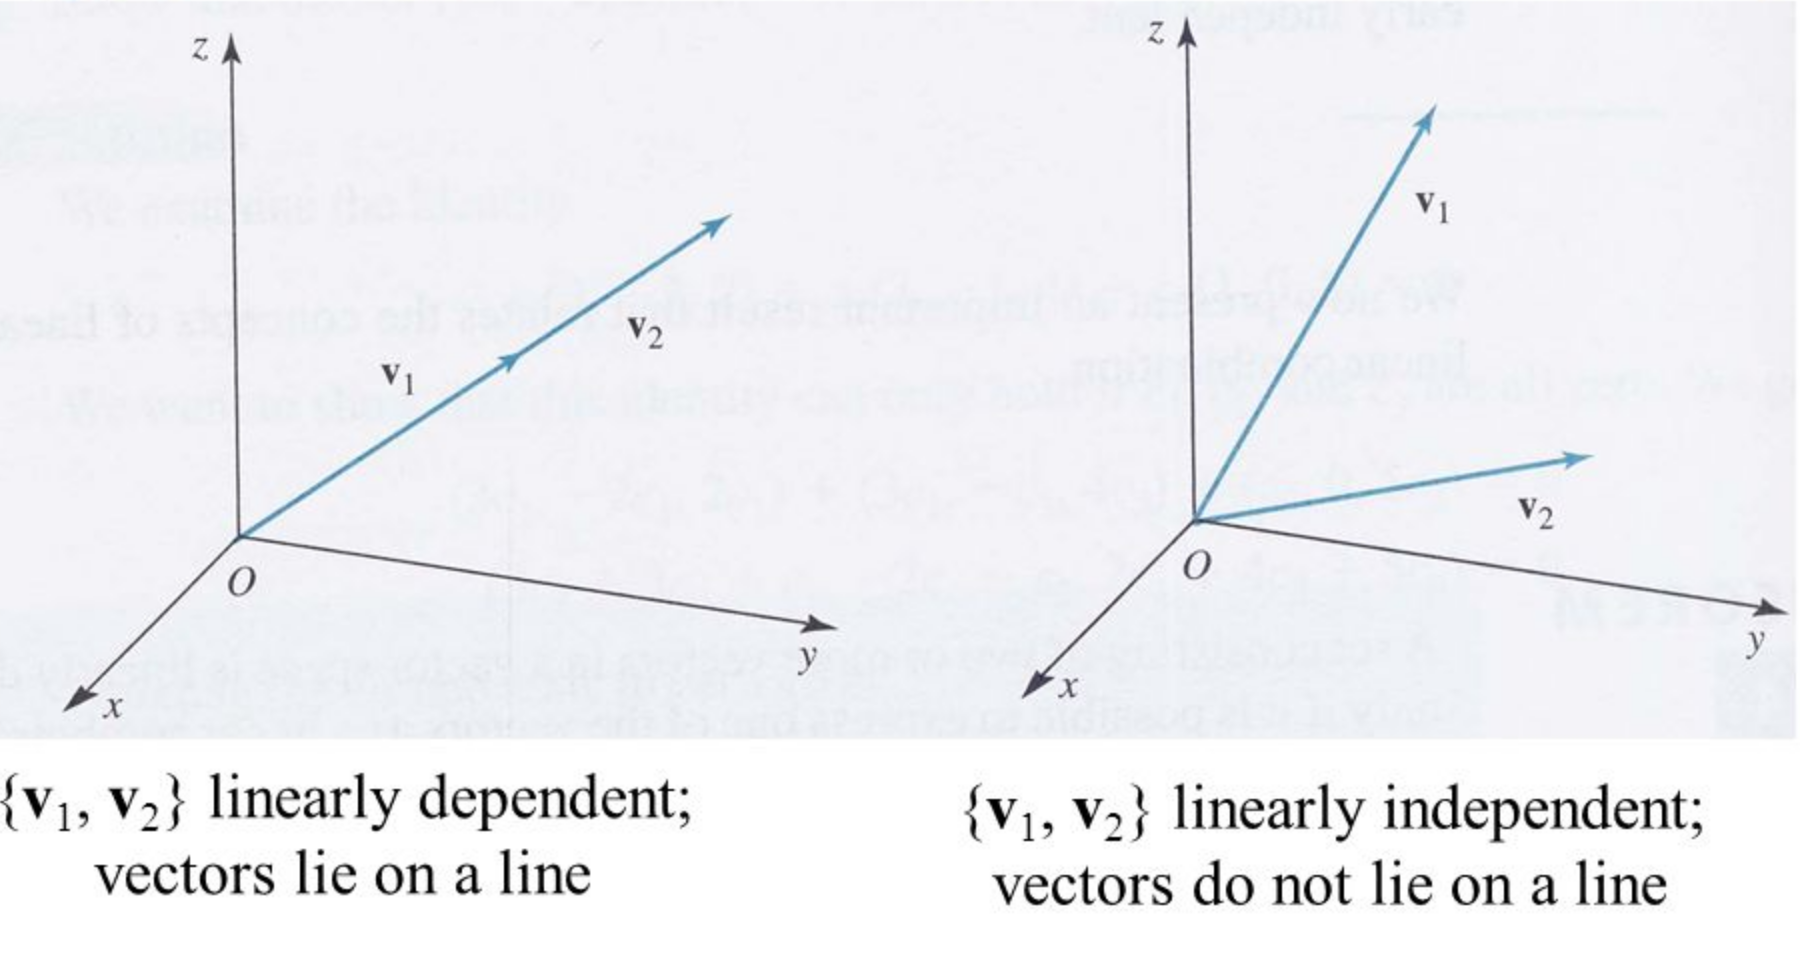
\includegraphics[width= \linewidth]{span_1.png}
\end{frame}

\begin{frame}{Column Span}
  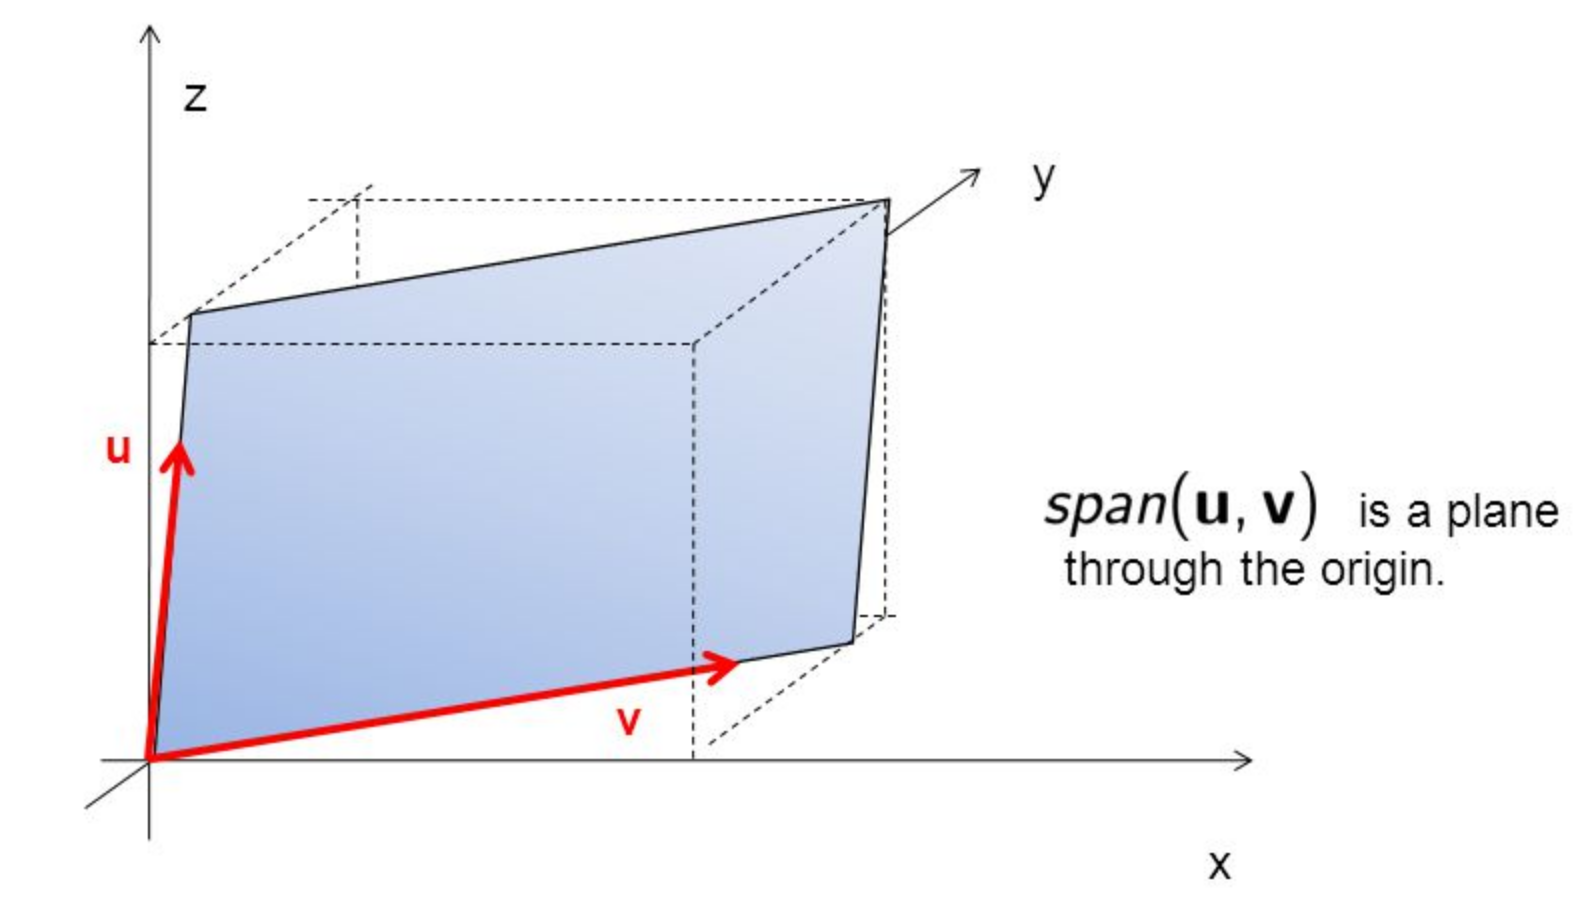
\includegraphics[width= \linewidth]{span_2.png}
\end{frame}

\begin{frame}{Column Rank of a Matrix}
  $$
    A = \begin{bmatrix}
      1 & 1 \\
      0 & 2 \\
      3 & 0 \\
    \end{bmatrix},
    B = \begin{bmatrix}
      1 & 2 \\
      0 & 0 \\
      3 & 6 \\
    \end{bmatrix}, \text{ and }
    C = \begin{bmatrix}
      1 \\ 0 \\ 0\\
    \end{bmatrix}
  $$
  \begin{itemize}
    \item The \alert{column rank} of a matrix is the number of linearly independent columns in a matrix (if two vectors are linearly dependent you only count one).

    \item $\text{rank}(A) = 2$, $\text{rank}(B) = 1$, and $\text{rank}(C) = 1$.
  \end{itemize}
\end{frame}

\begin{frame}{Finding Column Rank of a Matrix Practice}
  $$A = \begin{bmatrix}
      1 & 2 & 3 \\
      2 & 5 & 9 \\
      0 & 0 & 0
    \end{bmatrix}
  $$

  \vspace{50mm}
\end{frame}

\begin{frame}{Span Example}
  $$
    A = \begin{bmatrix}
      1 & 1 & 2 \\
      0 & 2 & 3 \\
      3 & 0 & 4
    \end{bmatrix},
    B = \begin{bmatrix}
      1 & 0 & 4 \\
      0 & 1 & 2 \\
      0 & 1 & 2
    \end{bmatrix}, \text{ and }
    C = \begin{bmatrix}
      1 & 0 & 0 \\
      0 & 1 & 0 \\
      0 & 0 & 1
    \end{bmatrix}
  $$
  \begin{itemize}
    \item Do matrices $A$, $B$, and $C$ span $\mathbb{R}^3$?
  \end{itemize}
  \vspace{50mm}
\end{frame}

% System of Equations
\section{Application 1: System of Equations}

\begin{frame}{System of Equations to Matrix}
  $$ 3x + y = 5$$ $$2x - y = 0 $$

  \begin{itemize}
    \item You can write system of equations in a matrix form:

          $$
            \begin{bmatrix} 3 & 1 \\ 2 & -1 \end{bmatrix} \begin{bmatrix} x \\ y \end{bmatrix} = \begin{bmatrix} 5 \\ 0 \end{bmatrix}
          $$
  \end{itemize}

  \vspace{30mm}

\end{frame}

\begin{frame}{Solving Systems of Equations using Matrices}
  $$
    \underbrace{\begin{bmatrix} 3 & 1 \\ 2 & -1 \end{bmatrix}}_{\equiv A} \begin{bmatrix} x \\ y \end{bmatrix} = \begin{bmatrix} 5 \\ 0 \end{bmatrix}
  $$

  \begin{itemize}
    \item By multiplying the matrix by its inverse, we can solve for $x$ and $y$:

          $$A^{-1} A \begin{bmatrix} x \\ y \end{bmatrix} = I_2 \begin{bmatrix} x \\ y \end{bmatrix} = \begin{bmatrix} x \\ y \end{bmatrix} = A^{-1} \begin{bmatrix} 5 \\ 0 \end{bmatrix}$$
  \end{itemize}

  \vspace{50mm}

\end{frame}

\begin{frame}{Solving System of Equations using Matrices}
  Solve the following: $$
    \begin{bmatrix} 3 & 1 \\ 2 & -1 \end{bmatrix} \begin{bmatrix} x \\ y \end{bmatrix} = \begin{bmatrix} 5 \\ 0 \end{bmatrix}
  $$

  \vspace{50mm}
\end{frame}


% Linear Regression
\section{Application 2: Linear Regression}

\begin{frame}{Linear Regression}
  \begin{itemize}
    \item In econometrics, we run a lot of regressions. We have a matrix of covariates $X$ and an outcome variable $y$.

    \item Our basic model is: $$
            y = X \beta + \epsilon
          $$, where $y$ is an $n \times 1$ vector, $X$ is an $n \times k$ matrix of $k$ variables, $\beta$ is a $k \times 1$ vector of coefficients, and $\epsilon$ is an $n \times 1$ vector of unobserved effect on $y$ (sum of the effect of other variables that affect $y$)

          $$
            X \beta = \begin{bmatrix} \underbrace{\vec{x_1}}_{n \times 1} &  \dots & \underbrace{\vec{x_k}}_{n \times 1}\end{bmatrix} \begin{bmatrix} \beta_1 \\ \vdots \\ \beta_k \end{bmatrix}
          $$
    \item $X \beta$ is just a linear combination of the explanatory variables.
  \end{itemize}
\end{frame}

\begin{frame}{Projection Matrix}
  Our regression coefficient is $\hat{\beta} = {\color{kelly} (X^T X)^{-1} X^T y}$ which is a matrix transformation applied to the vector $y$.

  \begin{itemize}
    \item When we want to predict $y$, we have $\hat{y} = X \underbrace{{\color{alice} (X^T X)^{-1} X^T y}}_{k \times 1}$ which is a linear combination of the columns of $X$.

    \item That is, the predicted values from a linear regression are just the $\vec{x_1} \hat{\beta}_1 + \dots + \vec{x_k} \hat{\beta}_k$

    \item We call the matrix $X (X^T X)^{-1} X^T$ the \alert{projection matrix} because it takes any vector and projects it to the span of $X$.
  \end{itemize}
\end{frame}




\end{document}
